% !TeX root = ./3-handout.tex

\setcounter{section}{2}
\section{Mathematical Induction \& Recursive Definitions}

\frame{  %\frametitle{Testing TOC}
 
 %\bigskip 
%\footnotesize{\tableofcontents}
\scriptsize{\tableofcontents}
%\setcounter{section}{2} %overwrites my slide counter and doesn't fix TOC anyways! 
}

%\iffalse 

\subsection{Intro to Math. Induction}

\frame{\frametitle{A Super-natural example!}
%\large
\begin{itemize}[<+->]

\item You're doing time in purgatory, and are automatically enrolled in philosophy (lucky you!)

\item Good news: To pass your class, you just need to produce one satisfactory piece of work

\item Bad news bears: your teacher is Gordon Ramsay, and he is never satisfied with any assignment

\item Whenever you turn something in, Ramsay returns it with suggestions for improvement, with revisions due tomorrow

\item How long should you expect to spend in this class?

\end{itemize}
}

%\iffalse %%%%%%%%%%%%%%%%%%%%%%%%%%%%%%%%%%%%%%%%

\frame{\frametitle{Mathematical Induction for SL Sentences}
%\large

If you want to prove that \emph{ALL} sentences (wffs) of SL have a particular property, it suffices to show the following:

\begin{enumerate}[<+->]

\item All \emph{atomic} sentences have that property (`\textbf{base case}')

\item If \metav{A} and \metav{B} are two \emph{arbitrary wffs} with that property, then so are the sentences built out of them by adding a connective \\ \hspace{4em} `\textbf{Induction step}' (There are five cases to consider:) 

\begin{enumerate}[(i)]
  \item $\enot \metav{A}$
  \item $(\metav{A}\eand\metav{B})$ 
  \item $(\metav{A}\eor\metav{B})$ 
  \item $(\metav{A}\eif\metav{B})$
  \item $(\metav{A}\eiff\metav{B})$

\end{enumerate}

%\item \textit{Induction Step}: assume antecedent of point 2

\end{enumerate}
}


\frame{\frametitle{A Simple Example}
\large
\begin{itemize}

\item Prove by induction that every well-formed formulae (wff) of SL has exactly as many left parentheses as it has \\ right parentheses

\item Don't forget to explicitly state the \textbf{base case}

\item Don't forget to explicitly state the \textbf{Induction Step}!

\end{itemize}
}

\frame{\frametitle{Three More Examples!}
\large

Prove the following by induction. Don't forget to explicitly state the base case and the induction step! 

\begin{enumerate}[<+->]

\item No wff begins or ends with a binary connective

\item No wff contains two consecutive binary connectives (i.e. with no symbols between them)

\item If a wff doesn't contain any binary connectives, then it is contingent. \normalsize{(hint: say that a wff is \textit{baller} if it either contains a binary connective or is contingent. Use induction to show that every wff is baller.)}

\end{enumerate}
}




\frame{\frametitle{Two DISTINCT notions of `Induction' }
%\large
\begin{itemize}[<+->]

\item \emph{Mathematical Induction} is completely different from \emph{scientific induction} or what we earlier called `inductive arguments' (which we contrasted with `deductive arguments')

\item \emph{Mathematical Induction}: Rigorous method of proving that a property holds for an infinite number of cases. Follow the steps we've outlined!

\item \emph{Scientific Induction}: fallible method of supporting a claim, based on a finite number of previous observations.

  \begin{itemize}[<+->]

\item All of the ravens I have ever seen are black

\item Therefore, the next raven I see will be black 

\item Notice how your conclusion could be wrong! Albino ravens!

\end{itemize} 

\end{itemize}
}

%\fi %%%%%%%%%%%%%%%%%%%%%%%%%%%%%%%%%%%%%%

%\iffalse

\subsection{Recursive Definitions}

\frame{\frametitle{A Non-recursive Motivation for Recursion} 
%\large
\begin{itemize}[<+->]

\item When a bigger thing can be studied in smaller chunks, it is often fruitful to do so

\item Descartes' \href{https://www.britannica.com/topic/Rules-for-the-Direction-of-the-Mind}{\textit{Rules for the Direction of the Mind}}: \\ break problems down to their simplest parts and have a secure grasp of them before proceeding

\item Or as we might say: Show me complexity, and I will find simplicity \\ (Gotta get this on a T-Shirt!)

\item Recursive definitions are one instance of applying this rule

\end{itemize}
}

\frame{\frametitle{A Non-recursive approach to Language Learning}
%\large
\begin{itemize}[<+->]

\item Some tourist manuals will have lists of sentences to phonetically memorize before travelling: learn how to say ``Where is the train to the airport?" or ``Where can one find a drugstore?" etc.\\

\item The plan is to commit all these to memory, by brute force.\\

\item You will know what ``Hvor er toget til lufthavnen", ``Hvor finder man et apotek?" etc. mean because you have seen them before and can recall them.\\
% these are sentences in Danish. `Where is the train to the airport'. `How to find a pharmacy?'

\item But this is entirely uncreative. You can only say/understand things you have seen before using this technique.\\

\end{itemize}
}

\frame{\frametitle{Recursion as the basis of English}
%\large
\begin{itemize}[<+->]

\item But much of the time, we say things that we've {\it{never}} said or heard before, yet we understand what they mean.\\
\bi

\item ``Your fate awaits in the office of the chair of \href{https://corporation.mit.edu/}{the Corporation}''
%\item ``The team's goaltender sold her tuba to pay her parking fines."  \\

\item I would bet no one in class has heard this sentence before.\\

\item But (maybe) you understand what it means.\\
\ei

\medskip 

\item What makes this possible is that our language has a recursive structure - we have basic components and then rules for making more complex, meaningful expressions out of them.\\


\end{itemize}
}

\frame{\frametitle{Example: Possessive of a noun phrase}
%\large
\begin{itemize}[<+->]

\item We can iterate grammatical rules, i.e. apply them again and again.\\

\item For example we have a way to form an expression \\ ``[Noun Phrase]'s son".\\

\item I can apply this to the name `Andrea' to get ``Andrea's son".\\

\item Then I can apply it again, to get ``Andrea's son's son".\\

\item And again, to get ``Andrea's son's son's son".\\

\end{itemize}
}

\begin{frame}
\frametitle{Example: nested object of verb phrases}

\begin{itemize}[<+->]
\item Sometimes, sentences can be so complicated that we need to break them down into components and study their structure to figure out what they mean

\item But if we understand the words, and we understand the rules of grammar, we can figure out the recursive structure

\item For example, the following is a meaningful sentence of English:

\item \textit{The rat the cat the dog bit chased ate the cheese}

\item What is this rat smoking??? It's not obvious that this is a meaningful sentence, never mind what it means!

\item []\end{itemize} 
\end{frame}

 \begin{frame}
\frametitle{Break it down!}

\begin{itemize}[<+->]
\item 
To figure out what it's saying, let's take a simpler part. Say that you see a rat eating some cheese.

\item You could say: ``The rat ate the cheese." Nothing obscure here 

\item But maybe there were several rats running around, and only one of them ate the cheese.

\item  You want to indicate which one, and it happens to be the one that the cat chased.

\item So you can form the noun phrase ``The rat the cat chased", and state ``The rat the cat chased ate the cheese."

\item  The rat $\underbrace{\Longrightarrow\Longrightarrow}_{\text{Which rat?}}$ The rat the cat chased\\

\end{itemize} 
\end{frame}

 \begin{frame}
\frametitle{Still breaking...}

\begin{itemize}[<+->]
\item 
And perhaps there are lots of cats running around too.

\item  You want to say specifically that you are referring to the cat that the dog bit.\\
 
  The cat $\underbrace{\Longrightarrow\Longrightarrow}_{\text{Which cat?}}$ The cat the dog bit.\\[3ex]
  
So take the phrase ``The rat the cat chased", and replace ``the cat" with ``the cat the dog bit" to get the noun phrase:

\item ``The rat the cat the dog bit chased":

\item And you can state that this particular rat, chased by that particular cat [the cat the dog bit] ate the cheese:

\item ``The rat the cat the dog bit chased ate the cheese."

\item []\end{itemize} 
\end{frame}

 \begin{frame}
\frametitle{More Examples of our Beautiful Recursive Language}

\begin{itemize}[<+->]
\item 

Now that you know the rules, and can apply them over and over, you can figure out what this means.

\item ``The rat the cat the dog the farmer bought bit chased ate the cheese." 

\item Some others to try for yourself (not essential to the course, for entertainment value only:)

\item 
%Bulldogs bulldogs bulldogs fight fight.\\ %i take it that `bulldog' is also a verb that means `wrestle', but i can't figure these out....
%Bulldogs bulldogs bulldogs fight fight bulldogs.\\
Fish fish fish fish fish. \\ %the penultimate fish is the verb 
Fish fish fish fish fish fish fish 
%middle fish is the verb, surrounded by `fish that fish fish' on both sides


\end{itemize} 
\end{frame}


%%%%%%%%%%%%%**********COOOL EXAMPLE FROM MACHINE LEARNING:************
% https://news.mit.edu/2022/ai-learn-patterns-language-0830

 \begin{frame}
\frametitle{A Moral of our Convoluted Story}

\begin{itemize}[<+->]
\item {\bf{The point}}: if you know the basic units (in this case: the words; in {\it{SL}} the sentence letters) and you know the rules for creating more complex meaningful parts, you open up an astonishing range of possibilities.


\item Definition by Recursion is the canonical way to define objects or structures that depend on iterated rules applied to a given basis

\item Proof by Induction is a powerful way to prove things about structures that are defined in this way. 

\end{itemize} 
\end{frame}

\subsubsection{Recursive Definitions for SL and $\mathbb{N}$}

\frame{\frametitle{Recursive Definition of Sentences of SL}
%\large

Recall that we define the well-formed formulae (wffs) \textit{recursively}: 
\begin{enumerate}[<+->]

\item \textbf{Base Clause}: Each atomic sentence is a wff 

\item \textbf{Recursion Clause(s)}: 

\begin{itemize}[<+->]

\item If $\metav{P}$ is a wff, then so is $\enot \metav{P}$

\item If $\metav{P}$ and $\metav{Q}$ are both wffs, then so are:

\begin{itemize}[<+->]

\item   $(\metav{P} \eand  \metav{Q})$

\item   $(\metav{P} \eor  \metav{Q})$

\item   $(\metav{P} \eif  \metav{Q})$

\item   $(\metav{P} \eiff  \metav{Q})$

\end{itemize}

\end{itemize}

\item \textbf{Closure clause}: Nothing else is a wff of SL


\end{enumerate}
}


\begin{frame}
\frametitle{Natural Numbers}

\begin{itemize}[<+->]

\item The set of natural numbers $\mathbb{N} = \{ 0, 1, 2, 3, 4, 5, \ldots \}$, beginning with $0$, is the
paradigm of a set of objects with a recursive definition.

\item The first natural number is $0$, and larger numbers are generated by adding $1$. 

\item Any whole number greater than $0$ can be reached by starting with $0$ and iterating this operation.  

\item (N.B.: Sometimes $\mathbb{N}$ is defined excluding `0'; \\ but remember: we are inclusive!!!)

\end{itemize} 
\end{frame}

\begin{frame}
\frametitle{Recursive Definition of ``natural number"}

\begin{itemize}[<+->]

\item Defining the set of natural numbers $\mathbb{N} = \{ 0, 1, 2, 3, 4, 5, \ldots \}$:

\item Put the definition into our fave recursion template:

\bi

\item {\bf{Base clause}}: 0 is a natural number.

\item {\bf{Recursion clause}}: If $n$ is a natural number then \\ \phantom{Recursion clausevv} $n+1$ is a natural number.

\item {\bf{Closure clause}}: Nothing else is a natural number.
\ei

\bigskip 

\item This definition generates the entire set $\mathbb{N} = \{ 0, 1, 2, 3, 4, 5, \ldots \}$, starting with 0 and repeating the operation of ``$+1$".

\end{itemize} 
\end{frame}


\subsubsection{Recursive definitions of Strings}


 \begin{frame}
\frametitle{Strings! (of letters---not of physics!)}

\begin{itemize}[<+->]

\item It can be useful to treat the set of {\it{all strings of letters}} in a given alphabet recursively

\item Say we take a fixed alphabet with just the characters $\{a, b\}$.

\item The basic strings will be the single characters $a$ and $b$.

\item  More complex objects are built up by the operation that inputs a string
$x$ and a member $u$ of the alphabet, and that outputs the string `$xu$' that results from appending `$u$' to the right of `$x$'

\item   Any string can be built up from a single letter by iterating this operation---in effect, simply spelling out `$x$' left-to-right. 

\end{itemize} 
\end{frame}

 \begin{frame}
\frametitle{An Example: Recursive Definition of Strings}

\begin{itemize}[<+->]
\item Let the alphabet be $\{a, b\}$ and consider the string `$bba$': \\ we obtain this string as follows:

\bi
 \item Start with `$b$'.  Append `$b$' to `$b$' and obtain `$bb$'  
 
 \item Finally, append `$a$' to `$bb$' and obtain `$bba$'
 
 \ei

\item Since we can generate every string this way, we can give a recursive definition of ``string of letters from the alphabet $\{a, b\}$":

\begin{enumerate}
\item {\emph{Base clause}}: $a$ and $b$ are strings from $\{a, b\}$

\item {\emph{Recursion clause}}: If $x$ is a string from $\{a, b\}$ then \\ \phantom{Recursion clausev} $xa$ and $xb$ are strings from $\{a, b\}$

\item {\emph{Closure clause}}: Nothing else is a string from $\{a, b\}$
\end{enumerate}
\end{itemize} 



\iffalse
\emph{Base clause}: The empty string $\epsilon$ is a string from $\{a, b\}$.\\
\emph{Recursion clause}: If $x$ is a string from $\{a, b\}$ then \\ \phantom{Recursion clausev} $xa$ and $xb$ are strings from $\{a, b\}$.\\
\emph{Closure clause}: Nothing else is a string from $\{a, b\}$.

\item 	Alternative: if you find ``the empty string" too abstract, we could omit it and give a different recursive definition
\fi 

\end{frame}



 \begin{frame}
\frametitle{Concatenation of the Feline Nation}

\begin{itemize}[<+->]
\item A note on terminology: when you stick together two strings of symbols, we say that you ``concatenate" them 

\item Sometimes, the symbol `$*$' is used to indicate concatenation, so ``$x*y$" means ``the result of concatenating the string $x$ and the string $y$".

\item Example: `$aaba*cca$' is just the string `aabacca'

\end{itemize} 
\end{frame}


%\subsubsection{Proofs in a formal system}

 \begin{frame}
\frametitle{Recursively Defining `Proofs'}

\begin{itemize}[<+->]
\item When we discuss metalogic, we will use the fact that {\it{proofs}} provide yet another domain that can be given a recursive definition

\item So the set of proofs is another domain where inductive arguments can be given

\item A generic description for now:

\item Proofs are constructed by applying rules of inference to premises

\item The simplest proofs are axioms or single premises:
\bi
\item Any axiom is itself a one-step proof of itself, a single premise is a one-step proof of itself, from itself. 
\ei
\end{itemize} 
\end{frame}

 \begin{frame}
\frametitle{Recursively Defining `Proofs'}

\begin{itemize}[<+->]

\item More complex proofs are built up from simpler ones by adding a step, which must either be an axiom or premise, or follow by a rule from earlier lines in the proof 

\item That is: something is a proof if it is an axiom or premise, or it is obtained from a proof by applying one of a finite number of rules!

\item So it's a recursive structure: A basis, iterated construction procedure, and nothing else:

%\item We can put this in our canonical form for recursive definitions: 

\begin{enumerate}
\item {\emph{Base clause}}: An axiom or a premise is a proof

\item {\emph{Recursion clause}}: If {\bf{Pr}} is a proof, then the result of applying one of the rules of our system [more on those later!] to make {\bf{Pr}} one line longer, is a proof

\item {\emph{Closure clause}}: Nothing else is a proof
\end{enumerate}

\end{itemize} 
\end{frame}




\subsection{Mathematical Induction}



 \begin{frame}
\frametitle{Mathematical Induction: Motivation}

\begin{itemize}[<+->]
\item One reason to pay attention to definition by recursion: it makes possible the proof technique of ``(mathematical) induction".

\item Don't confuse this use of `induction' with ``(scientific) induction", i.e. drawing probable inferences from observations (vs. ``deduction", which draws certain inferences by reasoning alone) %. That's a different use of the unfortunately ambiguous word ``induction".


\item We have inductive evidence that you'll be doing a lot of induction!

%If I were the ruler of the universe I would have required English to have two distinct words for these two distinct ideas, but nobody asked me....

\item 	Mathematical induction can be used in any domain where some objects can be singled out as basic, and where complex objects are built up out of simpler ones by iterating an operation.  


\end{itemize} 
\end{frame}



 \begin{frame}
\frametitle{General Pattern for mathematical induction for $\mathbb{N}$}

\begin{itemize}[<+->]

\item  If you can prove two facts (called the {\bf{Base case}} and the {\bf{Induction step}}) about a property C, then you know it holds for every natural number:

\bi

\item {\bf{Base case}}: C holds of 0. (or 1, or whatever you are starting the sequence with.)\\

\item {\bf{Induction Step}}: Assume that C holds of some given number $n$. (This assumption is called the {\it{Induction Hypothesis}}). \\ Using this assumption, prove that C holds of $n+1$.

\ei 

\bigskip

\item ALWAYS REMEMBER TO EXPLICITLY NOTE BOTH THE \emph{BASE CASE(s)} AND THE \emph{INDUCTION STEP}!

%\item We'll start with a simple use of induction on numbers, then consider more concrete cases.

\end{itemize} 
\end{frame}

\iffalse
 \begin{frame}
\frametitle{Non-math vs. Math Examples of Induction}

\begin{itemize}[<+->]
\item We can illustrate induction with a wide a range of examples, not just ones involving numbers.

\item These include physical systems and strings of letters

\item Hopefully this fights the misimpression that induction is only of use when dealing with the natural numbers $\mathbb{N}$. 

\item Nonetheless, there are particularly clean and simple examples arising from the natural numbers, and they will be useful for illustration too. 

\item If mathematical examples make you nervous, don't worry - this is just here for illustration.
\end{itemize} 
\end{frame}

\fi


\begin{frame}
\frametitle{A Simple Example of Induction over $\mathbb{N}$}

\begin{itemize}[<+->]
%\item I'll start here with a well-known example - you may have already seen it in high school algebra:

\item Prove that the sum of the first $n$ natural numbers is $\frac{1}{2}n(n+1)$ for any natural number $n$

\bi
\item (start at 1 and ignore 0, because it contributes nothing to the sum) 
\ei

%\item I'll discuss the problem a bit, and then give the proof, before dismantling it to study the moving parts. 

\item Some notation: to write a sum of a list of numbers, you need to index them to $1, 2, \ldots n$ to get a list $m_1, m_2, \ldots m_n$. Write this as:

\item $\displaystyle\sum_{i=1}^n m_i$  (using a capital greek `Sigma').\\[2ex]

\item Now it is particularly easy to write the sum of the first $n$ natural numbers: you don't need to index them to anything since they are in order already! 

\medskip

\item So just write: $\displaystyle\sum_{i=1}^n i = 1 + 2 + 3 + \ldots + n$

\end{itemize} 
\end{frame}

 \begin{frame}
\frametitle{Simple Example: checking some cases}

\begin{itemize}[<+->]
\item Often helpful to orient yourself by checking some cases:
%Now before we consider the problem in general, let's look around a little to orient ourselves.

\item Note that:\\
$1 =  \frac{1}{2} (1) (1+1) = \frac{2}{2} =1$

\item $1+2 =  \frac{1}{2} (2)(2+1) = 3$

\item $1+2+3 =  \frac{1}{2} (3)(3+1) =  (3)(2) = 6$

\item $1+2+3 + 4 =  \frac{1}{2} (4)(4+1) =  (2)(5) = 10$

%\item $\vdots$

Each of these is an instance of the formula  $\displaystyle\sum_{i=1}^n i =\frac{n(n+1)}{2}$\\[2ex]

\item When you try the formula in simple cases, it works. You might conjecture that it holds generally - but that isn't a {\it{proof}}.
\end{itemize} 
\end{frame}

 \begin{frame}
\frametitle{Simple Example: Motivating proof by Induction}

\begin{itemize}[<+->]
\item How can we prove that this formula holds generally?

\item Note this foothold: there is a way to break down each case so that it depends straightforwardly on the immediately previous one. 

\item Say that I ask you to compute $1+2+3 + 4 + 5$ and you already know that $1+2+3 + 4  = 10$

\item Note that $1+2+3 + 4 + 5 = \underbrace{[1+2+3 + 4]}_{\text{instance of prior case}} + \,\, 5 $\\[3ex]

\item Simplifies to $10 + 5 = 15$, given what you already know. 
%Not a big deal here, but it could be a real time-saver if you're dealing with 50 digit numbers! 

\end{itemize} 
\end{frame}

 \begin{frame}
\frametitle{Simple Example: Motivating proof by Induction}

\begin{itemize}[<+->]
\item Of course,  ``$1+2+3 + 4 + 5$'' is a small enough number that it's easy to just add the numbers together without bothering with simplifying tricks.

\item But with bigger numbers that becomes less and less of an attractive option. Using the simplifying trick saves loads of time.

\item It might take some time to add up the first 1,000,000 numbers, but if I already know the sum of the first 999,999, my job is easy: 

\item Just take {\it{that}} sum and add 1,000,000 to it!

%Or, more importantly, if you're dealing with an unspecified sum and you're looking for a pattern!

\end{itemize} 
\end{frame}

 \begin{frame}
\frametitle{An Inductive Proof of this Fact}

\begin{itemize}[<+->]

\item Now we want to \textbf{prove} the formula for the sum of the first $n$ numbers:

\item $\displaystyle\sum_{i=1}^n i =\frac{n(n+1)}{2}$

\item So we first need to prove the base case. In this problem, the base case is $n=1$.

\item So we've actually already covered the base case:

\item {\bf{Base Case:}}   $1 =  \frac{1}{2} (1) (1+1) = \frac{2}{2} =1$

%\item So we've taken care of that part.

\end{itemize} 
\end{frame}

 \begin{frame}
\frametitle{A Concern about the Induction Hypothesis}

\begin{itemize}[<+->]
\item For the Induction Step, we first {\bf{assume}} that we already know, \textit{for some given} $k$, that $\displaystyle\sum_{i=1}^k i = \frac{1}{2}k(k+1)$

\item We call this assumption ``{\it{The Induction Hypothesis}} (IH)".

\item At this point there may be howls from the bleachers: Isn't this just assuming what you have to prove??????

\item Good question! It shows you're paying attention. But no: it isn't assuming what you have to prove

\item In the IH, we could have even used `$n$' rather than `$k$'! 
 
 
\end{itemize} 
\end{frame}

 \begin{frame}
\frametitle{Induction Hypothesis}

\begin{itemize}[<+->]
\item What we want to prove is that the formula is true for every $n \in \mathbb{N}$. The induction hypothesis assumes we know the formula is true for some {\bf{specific}}, undetermined value $k$.\\
 
\item We will then {\bf{use}} the hypothesis to prove the case for $k+1$. 

\item We then {\bf{stop}} assuming the induction hypothesis, and instead conclude a conditional claim:

\item {\bf{If}} the induction hypothesis is true for a number $k$, {\bf{then}} the relevant property is also true for $k+1$

\end{itemize} 
\end{frame}

\begin{frame}
\frametitle{Induction Hypothesis}

\begin{itemize}[<+->]
\item 
Given the induction hypothesis, $\displaystyle\sum_{i=1}^k i = \frac{1}{2}k(k+1)$ we want to prove the formula holds for $k+1$, i.e. that:

\item  $\displaystyle\sum_{i=1}^{k + 1} i = \frac{1}{2}(k + 1)(k+2)$\\[3ex]

[{\bf{Note:}} We assume the formula is true for some number $k$, and we prove, {\it{given this assumption}}, that it must be true for $k+1$ as well.]

\end{itemize} 
\end{frame}

 \begin{frame}
\frametitle{Carrying out the Induction Step}

\begin{itemize}[<+->]
\item Our target is to show that $\displaystyle\sum_{i=1}^{k + 1} i = \frac{1}{2}(k + 1)(k+2)$ %\\[3ex]

\item OK, let's remember what we noted above, that:\\[2ex]

 $1+2+\ldots + (k+1) = \underbrace{[1+2+3 + \ldots + k]}_{\text{instance of prior case}} + (k + 1)$ %\\[3ex]

\item So we can simplify:  $1+2+3 +\ldots + (k+1) = [\frac{1}{2}k(k+1)] + (k+1)$ %\\[2ex]

\item Some algebra: [$\frac{1}{2}k(k+1)] + (k+1) = [\frac{1}{2}(k^2 +k)] + [\frac{2k}{2} + \frac{2}{2}$] %\\[2ex]

 \item[] $= \frac{k^2 + 3k +2}{2} = \frac{(k+1)(k+2)}{2} = \frac{1}{2}(k+1)(k+2)$
 
 \item And that's what we wanted to prove! 


%\item Now look up at the top. How about that! It's just what we were looking for!

\end{itemize} 
\end{frame}

\begin{frame}
\frametitle{Recapping the Structure of Our Inductive Proof}

\begin{itemize}[<+->]
%\item We conclude that, for every $n \in \mathbb{N}$, this formula holds: $\displaystyle\sum_{i=1}^n i = \frac{1}{2}n(n+1)$ %\\[3ex]

\item Recapping our Proof Steps (remember these steps!)

\begin{enumerate}

\item \emph{Base Case}: showed that $\displaystyle\sum_{i=1}^n i = \frac{1}{2}n(n+1)$ is true when $n=1$

\item \emph{Induction Step}: showed that for any $k$, {\bf{if}} $\displaystyle\sum_{i=1}^n i = \frac{1}{2}n(n+1)$ is true when $n = k$ {\bf{then}} 
$\displaystyle\sum_{i=1}^n i = \frac{1}{2}n(n+1)$ is true when $n = k+1$.

\end{enumerate}

\item These two facts entail that\\
 $\displaystyle\sum_{i=1}^n i = \frac{1}{2}n(n+1)$ when $n = {\textbf{any}}\,  k \in \mathbb{N}$, i.e. for all  $n \in \mathbb{N}$
 
\end{itemize} 
\end{frame}

 \begin{frame}
\frametitle{Why does Mathematical Induction Work?}

\begin{itemize}[<+->]
\item It's easy to see how this works: say we have a specific number. 

\bi 
\item To be concrete, say that I give you 325. 

\item How do you know that the formula holds when $n = 325$? 

\ei 

\item Well, the formula holds for $n=1$ (base case) and so by applying the induction step to the base case you know that the formula holds for $n=2$. Applying the induction step to $n=2$ tells you the equation holds for $n=3$ \ldots

\item Applying the induction step 324 times in this fashion gives you that the equation holds for $n=325$. 

 \item BOOM! 
 
 \bi 
 \item Feel that? That's the power of induction.  
 \ei 
 
 \end{itemize} 
\end{frame}


 \begin{frame}
\frametitle{A Non-inductive Proof of the Same Fact}

\begin{itemize}[<+->]
\item Here is a quick proof that, according to legend, the great mathematician Gauss found by himself when he was 7 years old

\item Take the sum  $\displaystyle\sum_{i=1}^n i = 1 + 2 + 3 + \ldots + n$ and write it twice, one above the other, the second one in the ``most to least" order, and add the series term by term. That is, %write and add:

\item  $\displaystyle\sum_{i=1}^n i = 1 + 2 + 3 + \ldots + n$\\
 {\underline{$\displaystyle\sum_{i=1}^n i = n + (n-1) + (n-2) + \ldots + 1$}}\\
 
\item[] $2 \times \displaystyle\sum_{i=1}^n i = \underbrace{(n+1) + (n+1) + \ldots (n+1)}_{n \text{ terms}} $ %\\[3ex]


\end{itemize} 
\end{frame}

 \begin{frame}
\frametitle{Non-inductive Proof Continued}

\begin{itemize}[<+->]

\item $2 \times \displaystyle\sum_{i=1}^n i = \underbrace{(n+1) + (n+1) + \ldots (n+1)}_{n \text{ terms}} $ %\\[3ex]

\item So we get $2 \times \displaystyle\sum_{i=1}^n i = n(n+1)$ and hence $\displaystyle\sum_{i=1}^n i =\frac{n(n+1)}{2}$

\item Which is what we were looking for, proved without induction

\item But notice how---in contrast to kid Gauss---induction doesn't require any special insight or inspiration! 

\end{itemize} 
\end{frame}

%OK, so these reflections can make it seem less mysterious, and the proof was quick and clear. But people like 5-year old Gauss don't come along every day. Until inspiration arrives, it's good to have %general techniques to rely on. And here we can break down the problem.

\subsubsection{Analogue of a HW Problem}

\begin{frame}
\frametitle{An Example to Work Through in Class!}

\begin{itemize}[<+->]

\item An analogue of a HW Problem: 

\item Prove that for all $n>3$, $n\in \mathbb{N}$, $2^n < n!$ \\[2ex] where $n! := \underbrace{(n \times (n-1) \times \ldots 3 \times 2 \times 1)}_{n \ times}$ \\[2ex] 

\item Just carry out the steps, noting each explicitly:
%. [This isn't a class on algebra, and so I'll just blip over the computations, which are a distraction.]

\item[] 1) What is the \emph{Base Case} we need to show?

\item[] 2) What is our \emph{Induction step}? \\ \phantom{vvv} i) Induction hypothesis?; ii) What do we need to show? 

\item[] 3) Just do it! (Note what you've proven)
%(99\% of the time, the base case is pretty trivial. Occasionally the conceptual realm throws us a curveball and the base case is harder than the induction step, but that is very rare.)

%note to class that we could have said `n greater than or equal to 4' (just like HW says n greater than or equal to five, so base case is n = 5)

\end{itemize} 
\end{frame}


\subsubsection{Sketch of another example (Skipped in Lecture)}

 \begin{frame}
\frametitle{An Example to Skip in Lecture!}

\begin{itemize}
\item Another numerical example with the same flavor (i.e. \textit{tasty}!) 
%I'm not going to cover this in lecture, but it is worthwhile to have another numerical example in the posted lecture overheads, for students who might find it helpful. If you don't think you'll find it illuminating, just cruise on by...

\item $\displaystyle\sum_{i=1}^n i^2 = \frac{1}{6}n(n+1)(2n+1) $%\\[2ex]

\item The general strategy for attacking this problem inductively:
%. [This isn't a class on algebra, and so I'll just blip over the computations, which are a distraction.]

\item[] 1) (\emph{Base Case}) prove $\displaystyle\sum_{i=1}^1 i^2 = \frac{1}{6}(1)(1+1)(2(1)+1) $%.\\[2ex]

\item Just elementary arithmetic (typically base cases are \textit{chill})
%(99\% of the time, the base case is pretty trivial. Occasionally the conceptual realm throws us a curveball and the base case is harder than the induction step, but that is very rare.)

\end{itemize} 
\end{frame}

 \begin{frame}
\frametitle{Another example continued}

\begin{itemize}

\item[] 2)  (\emph{Induction Step}): assume that for a given k, $\displaystyle\sum_{i=1}^k i^2 = \frac{1}{6}k(k+1)(2k+1)$\\[2ex]

\item Then set out to show that\\[2ex]

 $\displaystyle\sum_{i=1}^{k+1} i^2 = \frac{1}{6}(k+1)(k+2)(2(k+1)+1)$\\[2ex]

\item The trick is to find a way to {\it{use}} the information you are given in the induction hypothesis
\bi
\item Break down the $n=k+1$ case so it consists of the $n=k$ case plus some comparatively simple other stuff. 
\item This is usually the step that requires the most thought 
\ei 

\end{itemize} 
\end{frame}



 \begin{frame}
\frametitle{Working through the Deets}

\begin{itemize}
\item Happily, when we are dealing with sums, it is easy to simplify the $n=k+1$ case by appealing to the $n=k$ case:

\item[]  $\displaystyle\sum_{i=1}^{k+1} i^2 = \underbrace{1+2+3+ \ldots k}_{\text{This is} \sum_{i=1}^k i^2}  + (k+1)^2$\\[3ex]

\noindent $= [\sum_{i=1}^k i^2] + (k+1)^2$\\[3ex]

\noindent = $ \underbrace{\frac{1}{6}k(k+1)(2k+1)}_{\text{Substituting}\, {\frac{1}{6}k(k+1)(2k+1) \,\text{for}\, \sum_{i=1}^{k+1} i^2 }}+\, (k+1)^2$.\\[2ex]

Now we have an equation that doesn't have the sum operator in it at all. 

\end{itemize} 
\end{frame}

 \begin{frame}
\frametitle{Working through more Deets}

\begin{itemize}

\item[] \noindent = $ \underbrace{\frac{1}{6}k(k+1)(2k+1)}_{\text{Substituting}\, {\frac{1}{6}k(k+1)(2k+1) \,\text{for}\, \sum_{i=1}^{k+1} i^2 }}+\, (k+1)^2$.\\[2ex]

\item We now have a {\it{much}} simpler problem in front of us: 

\item Consider whether we can algebraically reduce $\frac{1}{6}k(k+1)(2k+1) +\, (k+1)^2 $ to\\[2ex] $\frac{1}{6}(k+1)(k+2)(2(k+1)+1)$.

\item Spoiler alert!

\item It is possible. (But I would not pay \$\$\$ for this show)

\end{itemize} 
\end{frame}

%\fi %*************************************************************************


\subsection{Ordinary vs. Complete Induction}

%use this subsection to transition to induction on strings, since complete induction is useful there! 

 \begin{frame}
\frametitle{Ordinary Induction vs. Complete Induction}

\begin{itemize}[<+->]
\item Proofs by mathematical induction fit into two slightly different schemes, depending on 
how much you assume in the induction hypothesis about the cases that are less complex than the one you set out to prove.

\item These argument patterns are equally rigorous, but they differ a bit in their logical structure, so it is worth pointing out the difference in form explicitly.

\item  In the cases we have just considered, we first prove some property is true of $0$ (or $1$, or whatever else is the first(s) in the series)

\item Second, we prove that if we assume that property is true of an arbitrary $n$,
we can prove it holds for the $(n + 1)$-th case %These two supports allow us to conclude that the property holds of every number.

\end{itemize} 
\end{frame}

 \begin{frame}
\frametitle{Complete induction (a.k.a. `strong induction')}

\begin{itemize}[<+->]
\item The variation is sometimes called the method of {\emph{complete induction}} (or `{\emph{strong induction}}').

\item  In complete induction, we modify the induction hypothesis:

\begin{enumerate}

\item We prove the base case as before

\item We assume that the property holds of {\emph{every}} number less than a given $k$ (adding the assumption that $k$ is greater than whatever number was considered in the base case)

\end{enumerate}
 
\item The difference is that instead of assuming the thesis {\it{just}} for the number preceding a given one, we assume it for {\emph{every}} number less than the given one

\item Each method is equally rigorous: it just happens that one form is convenient for some problems, the other for others
%but is that all! is there anything of intellectual significance!? e.g. diffs in EDRs

\end{itemize} 
\end{frame}



 \begin{frame}
\frametitle{Ordinary (a.k.a Weak) vs. Complete (a.k.a Strong) Induction}

%In terms of an argument template, here are the two forms:

%
%\item 

 \begin{block}<1->{Ordinary mathematical induction:}

{\bf{Base Case}}: $C(x)$ holds of the stuff in base clause, e.g. $0$

%0. [Or 1, or whatever the first element is in the given case.]\\
{\bf{Induction Step}}: Take any case $n$. If $C(x)$ holds of case $n$, then \phantom{{\bf{Induction Step}}:  } $C(x)$ holds of $n+1$
  \end{block}

\begin{block}<2->{\emph{Complete induction}:}

{\bf{Base Case}}: $C(x)$ holds of the stuff in base clause, e.g. `$a$' 

%$C(x)$ holds of 0. [Or 1, or whatever the first element is in the given case.]\\

{\bf{Induction Step}}: Take any $k >0$ [Or $k >$ the base case index(s)]. \\  \phantom{Induction Step} If $C(x)$ holds for \emph{every} $x < k$, then $C(x)$ holds of $k$.
  \end{block}

\begin{itemize}[<+->]
\item<3-> In both cases, if you can prove the Base Case and the Induction Step, you can conclude that $C(x)$ is true for every $x$ (yee haw!)
\end{itemize} 
\end{frame}


 \begin{frame}
\frametitle{A time to be Complete. A time to be Strong}

\begin{itemize}[<+->]
\item In particular: When dealing with strings of symbols in a language, the method of complete induction tends to be more useful. \\ 

\item Illustration: you are dealing with sentences in {\it{SL}}, doing induction on the number of connectives in the sentence %. (We will do this often in the middle part of the course.)

\item Say that $\metav{S}$ is a sentence with $n > 0$ connectives, and $\metav{S} = \metav{S}_1 \eor \metav{S}_2$.

\item Then you know that both $\metav{S}_1$ and $\metav{S}_2$ have fewer connectives than $\metav{S}$, but you don't know precisely how many either of them has.

\item The $n$ connectives in $\metav{S}$ could be divided up in lots of different ways between $\metav{S}_1$ and $\metav{S}_2$, so the hypothesis used in Complete Induction is more useful: it covers all the possibilities 

\item Language $SL$ says ``stay strong!''

\end{itemize} 
\end{frame}

%\fi %%%%%%%%%%%%%%%%%%%%%%%%%%%%%%%%%%%%%%%%%%%%%


\subsection{Recursion and Induction for Palindromes}

%some funny ones: https://www.grammarly.com/blog/16-surprisingly-funny-palindromes/

 \begin{frame}
\frametitle{Little Languages!}

\begin{itemize}[<+->]
\item One of the problems on the problem set is aimed at helping you get accustomed to doing induction/recursion on language structures 

\item In this case the ``language" is pretty rudimentary: the set of all strings you can make by concatenating the characters $\{a,b\}$

\item Let's spice things up by extending this alphabet to include the great big beautiful `c': $\{a,b,c\}$. 

%I talk about this case in the posted notes on recursion and induction, I'll go over the highlights here.

\item This is useful for providing a simple example of complete induction %I'll give an example of how to study a language using recursion and induction.

\end{itemize} 
\end{frame}

\begin{frame}
\frametitle{Palindromes  semordnilaP}

\begin{itemize}[<+->]
\item A \emph{palindrome} is a string of letters that reads the same way backwards and forwards (ignoring spaces and punctuation). One simple example is ``race car".

\item In case that example went by too fast: ``Yo, banana boy!'' ``Do geese see God?"

% More elaborate examples tend to sound a bit stilted, but they can be found. (``Nurse, I spy gypsies: run!; 
%``Go hang a salami, I'm a lasagna hog." \ldots)   
%from grammarly: Are we not pure? “No, sir!” Panama’s moody Noriega brags. “It is garbage!” Irony dooms a man—a prisoner up to new era.

\item  There are some trivial cases too: ``I" is an English language palindrome, and so is ``a". Aha! 
%For bookkeeping purposes let's count the empty string $\epsilon$ as a string of symbols. Then it's a palindrome also.

\item \textit{Let us turn now} to our rudimentary language of the set of all strings in the alphabet $\{a,b,c\}$, to study palindromes there

\item[] (We sometimes wonder: what if the reader said at this juncture, ``No! Thou shall not turn now!'' ?) 

%I will \textit{not} let you!''?)

\end{itemize} 
\end{frame}

 \begin{frame}
\frametitle{sthgisnI peeD (Deep Insights!)}

\begin{itemize}[<+->]
\item Say we want to prove things about palindromes \footnotesize{(and boy, do we ever!)}

\item Here is an insight that makes induction an option:

\item If you remove the first and last letter of a palindrome, you get {\it{another}} palindrome, two letters shorter \\ \centerline{($\Rightarrow$ \textit{insert mind-blown emoji here}$\Leftarrow$)} 

\item For instance: ``$aabbaabbaa$" is a palindrome. If you remove the first and last `$a$' then you get  ``$abbaabba$". \\ That's a palindrome too 
%(now you've got my attention)

\item  And so is ``$bbaabb$", etc, tracing right back to ``$aa$" 

\item[] \small{(tracing back even further, to the empty string `$\epsilon$', if we're string half-empty kinda people. `What's an empty string?' you might say:} \\ 

\item[] \small{oh, it's nothing)} 

\end{itemize} 
\end{frame}

 \begin{frame}
\frametitle{Recursively Defining Palindromes}

\begin{itemize}[<+->]
\item This mind-blowing fact lets us recursively define ``palindrome"

\item We can use the structure we've discovered to incorporate useful info about the set of palindromes into a recursive definition. 

\item Call a string over $\{a,b,c\}$ a \emph{recursive palindrome} if it satisfies the three conditions:

\begin{enumerate}
\item {\emph{Base clause}}: `$a$', `$b$', `$c$', `$aa$', `$bb$', `$cc$'  are recursive palindromes

\item {\emph{Recursion clause}}: If $s$ is a recursive palindrome, then $a*s*a$, \phantom{vvvvvvvvvvvvvv} $b*s*b$, and $c*s*c$ are recursive palindromes

\item {\emph{Closure clause}}: Nothing else is a recursive palindrome in $\{a,b,c\}$
\end{enumerate}

\end{itemize} 
\end{frame}


%need to edit following three and incorporate remarks on HW problem from Lect 5, 1.2.5

\begin{frame}
\frametitle{Induction over Palindromes}

\begin{itemize}[<+->]
\item What we want to do now is {\bf{prove}} that every palindrome in $\{a,b,c\}$ is a recursive palindrome, i.e. that our recursive definition captures the intuitive phenomena 
%The proof exploits the recursive structure of ``recursive palindrome" to give an inductive proof

\item We'll do induction on \textit{the length of a string} $s$

\item Note that what follows is NOT what you're being asked to do on PS 3, problem 1(ii). 

\item 1(ii) asks you to prove a specific property of a-palindromes 

\end{itemize} 
\end{frame}


\begin{frame}
\frametitle{Base Case of our Induction}

\begin{itemize}[<+->]

\item \emph{Base case:} Say that $s$ is 1 or 2 symbols long. Then:

\item[] i) it is one of `$a$', `$b$', `$c$', `$aa$', `$bb$', or `$cc$', in which case it is both a recursive palindrome and a palindrome

\item[] ii) It is one of `$ab$', `$ba$', `$bc$', `$cb$', `$ac$', or `$ca$' in which case it is neither a palindrome nor a recursive palindrome

\item (Argument for ii): None of the strings listed in ii) can be an R-palindrome because any R-palindrome that isn't called an R-palindrome by the base case must be called an R-palindrome by the recursion clause. 

\item[] --But if $s$ is an R-palindrome by the recursion clause, then it must contain at least three letters.)

\end{itemize} 
\end{frame}

%\iffalse 

 \begin{frame}
\frametitle{Stating the Induction Step}

\begin{itemize}[<+->]
\item \emph{Induction step}:
\noindent \textit{Assume} (Induction hypothesis) that every palindrome of length less than k symbols is a
recursive palindrome and conversely, where $k > 2$ %[that is: and the other way around]

\item Note that the ``and conversely" means we need to prove ``both directions" 

\item You WON'T need to prove both directions on your problem set! 

%($s$ a palindrome $\Rightarrow$ $s$ a recursive palindrome) Say that $s$ is a palindrome with exactly $k >2$ symbols.

%\item Since $s$ has three or more symbols, then we can remove the first and last letter, leaving a string $s'$. Since $s$ reads the same backwards and forwards, and $s'$ comes from $s$ by removing the first and last letter, $s'$ reads the same backwards as forwards. That is, $s'$ is a palindrome. Since $s'$ is a palindrome, and it has fewer than $k$ letters, then it is an inductive palindrome by the induction hypothesis.

%\item Since $s$ is a palindrome, the first and last letter must be the same, so it is either  `$a$', `$b$', or `$c$'. So $s$ = $a*s'*a$, or $s$ = $b*s'*b$, or $s$ = $c*s'*c$, where as we have shown $s'$ is an inductive palindrome. So, by the recursion clause of the definition of  inductive palindrome, $s$ is an inductive palindrome.

\end{itemize} 
\end{frame}

 \begin{frame}
\frametitle{Need to show: $s$ a palindrome $\Rightarrow$ $s$ a recursive palindrome}

\begin{itemize}[<+->]

%\item Induction Step: forwards direction

\item Let $s$ be an arbitrary palindrome with exactly $k$  symbols, $k >2$

\item Since $s$ has three or more symbols, we can remove the first and last letter, leaving a string $s'$. 

\item Since $s$ reads the same backwards and forwards, and $s'$ comes from $s$ by removing the first and last letter, $s'$ reads the same backwards as forwards. That is, $s'$ is a palindrome. 

\item Since $s'$ is a palindrome, and it has fewer than
$k$ letters, then it is an R-palindrome by the induction hypothesis

\item Since $s$ is a palindrome, the first and last letter must be the same, i.e. either 
`$a$', `$b$', or `$c$'. So $s$ = $a*s'*a$, or $s$ = $b*s'*b$, or \\ $s$ = $c*s'*c$, where as we have shown $s'$ is an R-palindrome. 

\item So, by the recursion clause of the definition of R-palindrome, $s$ is an R-palindrome.

\end{itemize} 
\end{frame}

\begin{frame}
\frametitle{NTS: $s$ a palindrome $\Leftarrow$ $s$ a Recursive palindrome}

%Finishing the Induction Step

\begin{itemize}[<+->]
\item Let $s$ be an arbitrary R-palindrome with exactly $k$ symbols, $k >2$

\item Since $k > 2$, $s$ cannot be an R-palindrome due to the base clause, so it must be counted by the recursion clause

\item Hence $s$ = $a*s'*a$, or $s$ = $b*s'*b$, or $s$ = $c*s'*c$, where $s'$ is an R-palindrome, by the recursion clause of the definition.

\item Since $s'$ has fewer than $k$ symbols, it falls in the scope of the induction hypothesis, so $s'$ is a palindrome. Since $s'$ is a palindrome, therefore $s$ = $a*s'*a$, or $s$ = $b*s'*b$, and $s$ = $c*s'*c$ are palindromes because they will also read the same backwards and forwards. 

\item Since one of these is $s$, $s$ is a palindrome

\item This completes the inductive proof. And so we ask ourselves: 

\item[] \small{Are we not pure? “No, sir!” Panama’s moody Noriega brags. “It is garbage!” Irony dooms a man—a prisoner up to new era.}

\end{itemize} 

\end{frame}


\subsubsection{Remarks on the ``a-palindrome" question on the problem set}

\begin{frame}
\frametitle{Remarks on the ``a-palindrome" question on the HW}

\begin{itemize}[<+->]
%\item More explicit roadmap for the ``a-palindrome" question on PS 3

\item Here's the problem:

\item Call a string over $\{a, b\}$ an ``a-palindrome" if it is a palindrome that has ``$a$" as the middle letter. 

\item (i) Give a recursive definition of ``a - palindrome", and \\ (ii) prove by induction that every a-palindrome has an even number of ``$b$"'s. 

\end{itemize} 
\end{frame}

\begin{frame}
\frametitle{Two things to do! (each with substeps)}

\begin{itemize}[<+->]
\item There are two things you need to do (each with substeps): 
%You have been given a definition of ``a-palindrome". You need to:

\begin{enumerate}

\item Give a recursive definition of ``a-palindrome". For ease of reference, say that the definition defines the ``recursive a-palindromes"

\item Using induction, show that every recursive a-palindrome has an even number of b's
\end{enumerate}

\item (In principle, you would also have to prove that the two definitions pick out the same set. That is, that a-palindromes are exactly the recursive a-palindromes. But I'm NOT asking you to do this as part of PS 3)

\end{itemize} 
\end{frame}

\begin{frame}
\frametitle{Modifying an Earlier Analogue problem}

\begin{itemize}[<+->]
\item Now step (1) is almost identical to the treatment of what are called ``recursive palindromes" above. In that more complicated case, focusing on alphabet $\{a,b\}$, we'd say: 

%In the notes I include the empty string as part of the definition though as I noted above, you have the option of dropping the empty string and giving this clause instead:


\begin{enumerate}
\item {\emph{Base clause}}: `$a$', `$b$', `$aa$', `$bb$' are recursive palindromes

\item {\emph{Recursion clause}}: If $s$ is a recursive palindrome, then $a*s*a$, \phantom{vvvvvvvvvvvvvv} and $b*s*b$ are recursive palindromes

\item {\emph{Closure clause}}: Nothing else is a recursive palindrome in $\{a,b\}$
\end{enumerate}


\item The definition of a-palindrome is {\it{almost identical}} to this. You really just need to modify one of the clauses

\item Then use induction to prove the claim about a-palindromes having an even number of ``b''s 

%\item Similarly the proof that every recursive a-palindrome is an a-palindrome, and conversely is a small modification of the proof given above. 


\end{itemize} 
\end{frame}

\subsubsection{Stamps}

\begin{frame}
\frametitle{Baby Stamps!}

\begin{itemize}[<+->]
\item Let's work through an analog of PS 3, problem 3
%You have been given a definition of ``a-palindrome". You need to:

\item \textsc{Baby Stamps}: prove by induction that if you have (an unlimited supply of) {2\textcent}  and {11\textcent}  stamps, you can make any integer amount greater than or equal to {10\textcent} 

\bigskip 

\begin{enumerate}

\item Base Case(s): more complicated than usual!

\item Induction Step: hint---use COMPLETE induction, so consider a specific $k > $ largest base case. Then state Induction hypothesis as holding for all $n$ less than $k$ but $\geq 10$ 
\end{enumerate}

%\item 

\end{itemize} 
\end{frame}

\begin{frame}
\frametitle{Hints for Question 4, PS 3}

\begin{itemize}[<+->]
\item Hint: the trick is to figure out \textit{what} to do induction \textit{over}!

%\item If you make a good choice, the induction step will parallel the base case

\item In the base case, consider two arbitrary odd numbers, and use the hint on the PS to express them (i.e. a natural number $d$ is odd if and only if there exists another natural number $k$ such that $d = 2k +1$). 

\item Use complete induction! 


%You have been given a definition of ``a-palindrome". You need to:

%\item 

\end{itemize} 
\end{frame}


%do hint for odd numbers problem; induction over number of factors 


\subsection{Recasting Induction in SL as Complete Induction} 

\begin{frame}
\frametitle{Special Induction Schema for the language {\it{SL}}}

\begin{itemize}[<+->]

\item Recall that for SL, we can use a special induction schema: 

\item If you want to prove that \emph{ALL} sentences (wffs) of SL have a particular property, it suffices to show the following:

\begin{enumerate}[<+->]

\item All \emph{atomic} sentences have that property (`\textbf{base case}')

\item If \metav{A} and \metav{B} are two \emph{arbitrary wffs} with that property, then so are the sentences built out of them by adding a connective \\ \hspace{4em} `\textbf{Induction step}' (There are five cases to consider:) 

\begin{enumerate}[(i)]
  \item $\enot \metav{A}$
  \item $(\metav{A}\eand\metav{B})$ 
  \item $(\metav{A}\eor\metav{B})$ 
  \item $(\metav{A}\eif\metav{B})$
  \item $(\metav{A}\eiff\metav{B})$

\end{enumerate}

%\item \textit{Induction Step}: assume antecedent of point 2

\end{enumerate}

%\item I want to give an example of complete induction for a claim about the language {\it{SL}} for sentential logic, since we'll be doing a bunch of that in the coming weeks.

%That is, it's just the part of {\it{SL}} that has atomic sentences, parentheses, and ``\&".

\end{itemize} 
\end{frame}


\begin{frame}
\frametitle{Complete Induction for the language {\it{SL}}}

\begin{itemize}[<+->]
\item Implicitly, this special schema is Complete Induction over the string length $k$ of an SL sentence

\item To simplify, let's use a fragment of {\it{SL}} that contains just atomic sentences and sentences whose only connective is ``$\&$''

\item We can use induction because this rudimentary part of {\it{SL}} has a recursive definition:

\begin{enumerate}
\item {\emph{Base clause}}: Every atomic sentence is a sentence of {\it{SL}}

\item {\emph{Recursion clause}}: If \metav{P} and \metav{Q} are sentences of {\it{SL}}, then $(\metav{P} \eand \metav{Q})$ is a sentence of {\it{SL}}

\item {\emph{Closure clause}}: Nothing else is a sentence of (our fragment of) {\it{SL}}
%unless it results from application of the recursion clause to the expressions specified in the base case.
%, except what you get by beginning with $aab$ and repeatedly applying the Recursion Clause
\end{enumerate}

\end{itemize} 
\end{frame}

\begin{frame}
\frametitle{Complete Induction for the language {\it{SL}}}

\begin{itemize}[<+->]

\item Let's reprove this claim (for our fragment): every sentence of SL has an equal number of left and right parentheses
%\item Every sentence $S$ in this language has the same number of right as left parentheses, namely 0.

\item Proceed by (complete) induction on the number $n$ of symbols in the sentence \metav{S}, i.e. the string-length:

\item {\bf{Base Case}}: $n=1$

\item[] Then \metav{S} is an atomic sentence, so it has no parentheses. Thus there are the same number of right and left parentheses.

\end{itemize} 
\end{frame}

\begin{frame}
\frametitle{Starting the Induction step}
\begin{itemize}[<+->]
\item {\bf{Induction step}}: Let \metav{S} be an arbitrary sentence of SL with $k$ symbols, where $k>1$. Assume that  every sentence of this language with fewer than $k$ symbols has the same number of left as right parentheses (Induction hypothesis)

\item \metav{S} is not a sentence letter, so it must be of the form $(\metav{S}_1 \eand \metav{S}_2)$, with $\metav{S}_1$ and $\metav{S}_2$ sentences of {\it{SL}} (since we're focusing on the conjunctive fragment of SL)

\item Note that $\metav{S}_1$ and $\metav{S}_2$ have fewer than $k$ symbols 

\item So by the induction hypothesis, both $\metav{S}_1$ and $\metav{S}_2$ have the same number of left and right parentheses

\item (Note that we can't assign a specific length to $\metav{S}_1$ or $\metav{S}_2$. We just know that the length of each is less than $k$. That's why we use complete induction rather than ordinary induction in this case)

\end{itemize} 
\end{frame}

\begin{frame}
\frametitle{Finishing the Induction Step}

\begin{itemize}[<+->]
\item So the total number of right parentheses in $\metav{S}$ is:

\item[] 1 + (number of right parentheses in $\metav{S}_1$) + (number of right parentheses in $\metav{S}_2$)

\item And the total number of left parentheses in $\metav{S}$ is:

\item[] 1 + (number of left parentheses in $\metav{S}_1$) + (number of left parentheses in $\metav{S}_2$).

\item These two numbers must be equal, since they are sums of three numbers, each number equal to its counterpart in the other sum

\item This completes the induction step, and so the proof.

\end{itemize} 
\end{frame}

\begin{frame}
\frametitle{Remarks of a common-sensical nature}

\begin{itemize}[<+->]
\item Of course, what we just proved by induction is a piece of common sense:

\item {\it{Of course}} there will be the same number of left as right parentheses, since the only way for a parenthesis to get into a formula is to get there by an application of the recursion clause, and the recursion clause just adds exactly 1 of each type of parenthesis, every time.

\item The point is not that this is a hard problem but rather that it is so simple that it helps make clear how common-sensical the inductive pattern of reasoning is, when it isn't bound up with other complications

\end{itemize} 
\end{frame}


\begin{frame}
\frametitle{Wise Words, from our hero Frege}

\begin{itemize}[<+->]
\item Gottlob Frege---who worked out most of the core ideas in the modern approach to logic---wrote in 1884:

\begin{quote} 
If, by examining the simplest cases, we can bring to light what humankind has there done by instinct, and extract from such procedures what is universally valid in them, may we not thus arrive at general methods for forming concepts and establishing principles that will be applicable in more complicated cases? ({\it{Foundations of Arithmetic}} \S2)
\end{quote}

\item And that's what we've often done above: take common sense cases and extract a general pattern we can use in more complicated cases, where the answers are not so obvious.

\item Sensing strong Descartes-energy here 
%\item END DETRITUS}

\end{itemize} 
\end{frame}


\subsection{More induction and recursion on strings}

%\subsubsection{$aab$ strings - the common sense version}

\begin{frame}
\frametitle{$aab$ strings: a common sense version}

\begin{itemize}[<+->]
\item Another example of a proof by induction so simple that you might think it silly to spell it out

\item We deal again with a ``language" we know and love: all strings of letters from the alphabet $\{a,b\}$.

\item Call a string in this language an `$aab$-string' if it consists of nothing but a series of the letters $aab$ repeated some number of times.

\item So $aab$, $aabaab$, $aabaabaab$, $aabaabaabaab$, \ldots  are $aab$-strings.

\end{itemize} 
\end{frame}

\begin{frame}
\frametitle{A Radical Claim}

\begin{itemize}[<+->]
\item I now claim that any $aab$-string has more $a$'s in it than $b$'s

\item Your reaction might be ``Can you believe this guy? Back at it again with the trivial examples. {\it{Of course}} there are more $a$'s than $b$'s in an $aab$-string."

\item ``In fact, there will always be exactly twice as many $a$'s as $b$'s. That's {\it{obvious}} from the definition!"

\item When you say this, you are implicitly using recursive/inductive reasoning

\end{itemize} 
\end{frame}

\begin{frame}
\frametitle{Heuristic Recursive Reasoning (not a proof!)}

\begin{itemize}[<+->]
\item We spell out what is implicit in the ``it's obvious" reaction. Sometimes our common-sense reactions can have more hidden logical intricacy than we realize 

\item (often, things are not what they seem. Consider the dark underbelly of suburbia) 
%david lynch 1986 Blue Velvet; not sure if Lynch after said these lines though...

\item One way to look at it is this: You get $aab$ strings by repeatedly sticking $aab$'s together

\item Each time you stick on a new $aab$ you add one $b$ and two $a$'s. And you start out with more $a$'s than $b$'s in $aab$, the shortest $aab$-string.

\item There's no way to get more $b$'s than $a$'s with that process, no matter how many times you repeat it.

%\item (That's the principle behind the old joke: A:``I lose money on every car I sell" B:``Then how can you stay in business?" A:``I make it up with volume sales!")

\end{itemize} 
\end{frame}

%\subsubsection{$aab$ strings - Translating common sense into inductive argument}

\begin{frame}
\frametitle{Translating common sense into an inductive argument}

\begin{itemize}[<+->]
\item To translate the common sense reaction, we first make explicit---using recursion!---the idea that $aab$-strings are built up by successively adding $aab$:

\begin{enumerate}
\item {\emph{Base clause}}: $aab$ is an $aab$-string

\item {\emph{Recursion clause}}: If $s$ is an $aab$-string, then $s*aab$ is an $aab$-string

\item {\emph{Closure clause}}: Nothing else is an $aab$-string in $\{a,b\}$
%, except what you get by beginning with $aab$ and repeatedly applying the Recursion Clause
\end{enumerate}

\item Next, use the fact that the $aab$-strings are built up this way to argue \emph{by complete induction on string length} that they must have more $a$'s than $b$'s

%\item {\bf{NOTE: This is just for the sake of the illustration. For the problem sets, you don't have to explicitly state recursive definitions before you apply induction unless you are specifically asked to state them.}}

\end{itemize} 
\end{frame}

\begin{frame}
\frametitle{Starting the Inductive Proof on $aab$-strings}

\begin{itemize}[<+->]
\item \emph{Base Case}: $aab$ has more $a$'s than $b$'s

\item \emph{Induction Step}: {\it{Assume}} that for any arbitrary $aab$-string $s$ with fewer than $k$ letters (where ($3<k$) ), the property holds, i.e. that this string $s$ has more $a$'s than $b$'s.
% that if $s$ is an arbitrary $aab$-string with fewer than $k$ letters, ($3<k$) then $s$ has more $a$'s than $b$'s. 

\bi

\item this is our `Induction Hypothesis' for Complete Induction

\item **Note - we need to make $k$ greater than 3, because the string in the base case has 3 letters

\ei

\bigskip

\item Try to finish the proof yourself before flipping to next slide! \\ Hint: consider an arbitrary $aab$-string $t$ with $k$ letters. 



\end{itemize} 
\end{frame}

\begin{frame}
\frametitle{Finishing the Induction Step for $aab$-strings}

\begin{itemize}[<+->]

\item Let $t$ be an arbitrary $aab$-string with exactly $k$ letters

%\medskip

\bi

\item Since $3<k$, that means that $t$ cannot be $aab$, so it must have been produced by some applications of the recursion clause

\item That means that there is some other $aab$-string $t'$, such that $t = t'* aab$.

\ei

\medskip

\item $t'$ is three letters shorter than $t$ so it has fewer than $k$ letters

\bi

\item Since it has fewer than $k$ letters it falls within the scope of the induction hypothesis, and so it has more $a$'s than $b$'s.

\item Since $t$ has two more $a$'s and only one more $b$ than $t'$, that means $t$ has more $a$'s than $b$'s as well.

\ei 

\medskip

\item This completes the induction step and hence the proof

\end{itemize} 
\end{frame}



%\iffalse

%***********************************************************************************
\subsection{Extra `Big Picture' stuff for Recursion}

 \begin{frame}
\frametitle{Defining `Definition'}

\begin{itemize}[<+->]
\item What do we want a definition to do? 

\item We want to give meaning to a word that previously had no meaning, and we want it to do it in a way that allows a person who didn't previously know what the word meant to come to know what it means.

\item Simple example: I introduce a new word into our vocabulary: grunsk. What does it mean? Well, something is grunsk if and only if it is a blue volleyball. 

\item OK, you might not see much point to having a word like this, but the definition does allow you to use it. All you need to now is what `` is a blue volleyball" means, and you can confidently divide the world into the grunsks and not-grunsks. 
\item[] \end{itemize} 
\end{frame}

 \begin{frame}
\frametitle{Ways to \#fail: e.g. Circular Definitions}

\begin{itemize}[<+->]
\item 
There are ways that this pattern can screw up: it might be that the words are too vague, or perhaps they don't pick out a unique thing or class. 

\item Another way a definition can fail is if it is circular, such as: ``Something is grunsk if and only if it is a blue grunsk." 

\item That definition doesn't do what it's supposed to do.\\
% It's not completely devoid of information: Before you didn't know anything about grunsks, and now at least you know they %are orange.

\item Say I hand you a blue thing and ask you if it is a grunsk. You can't use the definition to decide unless you already know what a grunsk is. 

\item Let's say you hear this and you say to yourself: OK I've been warned. No circular definitions for me, thank you very much.

\item How to spot them so you can avoid them?
\item[] \end{itemize} 
\end{frame}

 \begin{frame}
\frametitle{A Guideline to Avoid Circularity}

\begin{itemize}[<+->]
\item This looks like a good guideline: set the word you want to define on a specific side of the definition (usually it's the left hand side, but our recursive definition has the word to be defined on the right). Then if the word also occurs on the {\it{other}} side, the definition is circular.

\item And usually, that's a trustworthy guideline. But not in the case of recursive definitions. In this case things are more subtle.

\item I'll continue with the definition of our SL wffs and then revisit the point.


%\item We've had a bit of a digression, so let's remind ourselves where we were:

\end{itemize} 
\end{frame}

 \begin{frame}
\frametitle{The Base Clause}

\begin{itemize}[<+->]
\item First the Base clause: Every atomic sentence is a wff/sentence. 

\item You might think there is some circularity here: Isn't the word ``sentence" on both the right and the left side, at least when we call `wffs' `sentences'? 

\item But ``atomic sentence " is a defined expression: we defined it by listing the capital letters of the English alphabet, allowing subscripts from the natural numbers

\item You don't need to know what the word ``sentence" means to understand what an atomic sentence is from this definition.

%\item To illustrate, say that we used the expression ``Basic letter" rather than ``sentence letter". 

%\item The clause ``Every basic letter is a sentence." doesn't even have this appearance of circularity.
\end{itemize} 
\end{frame}

 \begin{frame}
\frametitle{The Whole as Distinct from its Parts}

\begin{itemize}[<+->]
\item 
It can happen that we understand what an expression as a whole means, even if we don't understand the parts

\item (Most of us understand what ``hoist with his own petard" means, (like many clich\'es, this is a turn of phrase originally introduced by Shakespeare) even though we misunderstand the relevant meaning of ``hoist", and we don't know what a ``petard" is.)

%Aside: Fun Fact: This is a residue of French in English: p\'etard and ``p\'eter" (fx. ``les plombs")); French had a great %influence on Shakespeare's English. Until about a century earlier every English king had been a native French speaker, since %1066 AD.

\item In the words of the philosopher Quine: such occurrences of words are like ``cat" in ``cattle" - you don't have to understand ``cat" to know what cattle are.

\item  You don't have to know what ``sentence" means to understand the stipulation: The {\it{atomic sentence letters}} are the capital Roman letters in the English alphabet, with or without number subscripts.

\end{itemize} 
\end{frame}




\subsection{Towers of Hanoi Example} 

 \begin{frame}
\frametitle{Towers of Hanoi }

\begin{itemize}[<+->]

%\item (See the posted ``towers-of-hanoi.pdf" slides)

\item As a concrete, non-mathematical example, we'll consider a puzzle
that looks at first as if it might be very hard, but it becomes simple and straightforward if we think about it in terms of recursion.

\item This is a tabletop puzzle called the \emph{Towers of Hanoi}. 

\item You are given three pegs and $n$ discs. No two discs are the same size. 

\item At the beginning of the game, all $n$ discs are all on the leftmost peg, with the largest disc on the bottom, and then the remaining discs in decreasing order of size piled on top of the first, with the smallest on top.

%\item Here is a drawing of the opening setup in the case of 6 discs %:\\[4ex]

\end{itemize} 

%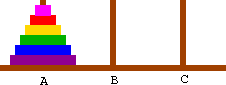
\includegraphics{Hanoi_n_6_png.png}
\end{frame}

 \begin{frame}
\frametitle{Towers of Hanoi: Initial State}

\begin{itemize}[<+->]

\item Given three pegs and $n$ discs. No two discs are the same size. 

\item Initial state: all $n$ discs are all on the leftmost peg, with the largest disc on the bottom, and then the remaining discs in decreasing order of size piled on top of the first, with the smallest on top.

\item Here is a drawing of the opening setup in the case of 6 discs %:\\[4ex]

\end{itemize} 

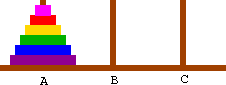
\includegraphics{Hanoi_n_6_png.png}
\end{frame}

 \begin{frame}
\frametitle{Towers of Hanoi: Goals and Rules}

\begin{itemize}[<+->]
\item Goal: end up with all discs on the right peg, in the same order, that is, smallest on top, and increasing in size towards the bottom.

\item There are restrictions on how the discs are moved:
\begin{enumerate}
\item The only allowed type of move is to take \emph{one} disc from
  the top of a pile and drop it on another peg. 
  \item Moving several discs at once is not allowed.
\item A larger disc can never lie above a smaller disc, on any peg.
\end{enumerate}

\end{itemize} 
\end{frame}

 \begin{frame}
\frametitle{Towers of Hanoi}

\begin{itemize}[<+->]
\item 
Question: Is it possible to solve the puzzle for any number of discs?

\item It turns out that by thinking recursively, we can find a very simple answer.

\item If you haven't already read the notes, try experimenting with the puzzle to see what you think.

%\item There is an online version at at this wonderful children's site:

\item There is an online version at \href{https://www.mathsisfun.com/games/towerofhanoi.html}{Math is Fun!}


\end{itemize} 
\end{frame}

%\fi 




\iffalse 

%***********************ADDITIONAL EXAMPLES FROM JTAPP 303 LECTURE 5****************
%******************Fibonacci and Sum of first n Odd Numbers****************************
%NB: would need to edit slides
%this material could be useful if I want to drag out induction to three days, or if i want to include the practice problems above for recitation sections and swap in material below for lecture! 



 \subsubsection{Multiple cases in the Base Case/Clause; Fibonacci numbers}

\begin{frame}
\frametitle{Ethics}

\begin{itemize}[<+->]
\item Usually, the base case of a mathematical induction, and the base clause of a recursion, will cover one case only.
\item  
But this isn't always true: sometimes the recursion is generated after beginning with two or more cases that are defined independently.

\item Here is an example to illustrate that sometimes the base case of a recursion / induction can involve more than one special case.

\item {\bf{NB: The problem set has a question about stamps that will require you to cover several cases in the Base step.}}

\end{itemize} 
\end{frame}


\begin{frame}
\frametitle{Ethics}

\begin{itemize}[<+->]
\item 
A sequence of numbers that shows up in a surprising number of places in nature is the Fibonacci sequence:

\item \medskip

1,1,2,3,5,8,13,21,34,...

\item \medskip

\noindent Each number in the sequence is the sum of its two predecessors.

\item The inductive definition of this one
is a bit different from the ones we are used to, since there are {\bf{two}} independently specified starting points, and we need to consider both $f(k)$ and $f(k-1)$
to define $f(k+1)$:

\item \noindent $f(0) = 1$ 
\item $f(1) = 1$ 
\item $f(n+1) = f(n-1) + f(n)$ for $n>1$

\item 
\end{itemize} 
\end{frame}



\begin{frame}
\frametitle{Ethics}

\begin{itemize}[<+->]
\item 
\noindent As usual, the inductive structure makes it possible to prove things.

\item Here's a very simple question to illustrate: is the Fibonacci function $f$ we've just defined dominated by the exponential function $g(x) = 2^x$?

\item That is, is it always the case that  $f(x) \leq g(x)$?

\item Aside: It's not any harder to prove the strict equivalence $f(x) < g(x)$ (except for the case $f(0) \leq g(0)$) but since this example is meant for illustration, I want to keep the argument structure simple.  

\item 
\end{itemize} 
\end{frame}


\begin{frame}
\frametitle{Ethics}

\begin{itemize}[<+->]
\item 
 It's easy to confirm this for the base cases:

\item \medskip

\noindent $f(0) = 1 = 2^0 = g(0)$ and
\item \noindent $f(1) = 1 < 2 = 2^1 = g(1)$

\item \noindent But once you've taken care of these specific cases, how can you go on? 

\item %\end{itemize} 
\end{frame}


\begin{frame}
\frametitle{Ethics}

\begin{itemize}[<+->]
\item 
The basic observation is simple: use the elementary fact that if
$a \leq c$ and $b \leq c$ then $a + b \leq 2c$.

\item This tells us that repeatedly taking fibonacci numbers is not going to pull ahead of repeatedly multiplying by two. %Try it for the first seven or so values of each sequence:

\item %1,1,2,3,5,8,13...

\item %\medskip

%1,2,4,8,16,32,64,...

\end{itemize} 
\end{frame}


\begin{frame}
\frametitle{Ethics}

\begin{itemize}[<+->]
\item The inductive argument is the way to make this informal idea rigorous. 

\item 

We have already proven the {\bf{Base Case}} for $f(0)$ and $f(1)$.

\item Now we {\bf{Assume}} (Induction Hypothesis) that for every n such that $1 < n < k$,
$f(n) \leq 2^n$. 

\item We want to show $f(k) \leq 2^k$. 

\item This follows immediately from the facts that (by the induction hypothesis):

\item $f(k-1) \leq 2^{k-1}$ and

\item $f(k-2) \leq  2^{k-2} (< 2^{k-1})$

\item Apply this instance of the ``elementary fact'' from above:
$f(k) = f(k-2) + f(k-1) \leq 2^{k-1} + 2^{k-1} = 2 \times 2^{k-1} = 2^k$.

\item \noindent This proves the induction step, so we're done.


\end{itemize} 
\end{frame}




\subsubsection{Another Series: Adding the Odd Numbers}

\begin{frame}
\frametitle{Ethics}

\begin{itemize}[<+->]

\item Here is another problem that involves adding numbers.

\item The algebra here is particularly simple, and it illustrates an important point -- sometimes you need to analyze and restructure a problem before you can apply induction to it.

\item {\bf{Part of the reorientation involves a hint used in the last question on the problem set, about products of odd numbers.}}

\end{itemize} 
\end{frame}


\begin{frame}
\frametitle{Ethics}

\begin{itemize}[<+->]
\item 
The problem: Find a formula for the sum of the first $n$ odd numbers.

\item That is, we want a formula that will tell us how much each of these sums is (among others):

\item $1+3 = ?$
\item $1+3+5 = ?$
\item $\vdots$
\item $1+3+5+7+9+11 = ?$
\item $\vdots$
\item $1+3+5+7+9+11+13+15+17 = ?$
\item $\vdots$

\end{itemize} 
\end{frame}


\begin{frame}
\frametitle{Ethics}

\begin{itemize}[<+->]
\item 

Now as I mentioned there is a preliminary question we should address. The simplest pattern of recursive arguments comes when we can order things like the natural numbers, with a first, a second, a third, \ldots

\item We want a simple way to configure this series so that for each natural number $n$, some term in the series is counted as the $n$'th (and only one term gets counted as the $n$'th)

\item 
\end{itemize} 
\end{frame}


\begin{frame}
\frametitle{Ethics}

\begin{itemize}[<+->]
\item 
This is easy to do if you note that the $i$'th term in the series of odd numbers is $2i - 1$:

\item 2(1) - 1 = 1 
\item 2(2) - 1 = 3 
\item 2(3) - 1 = 5 
\item \vdots

\item So we can put our question this way:

\item What is a formula for this sum: $ \sum\limits_{i=1}^n 2i - 1 $?

\item Which is another way of saying: 

\item What is the formula for $1+3+5+ \ldots + [2(n-1) - 1] + [2n - 1]?$

\end{itemize} 
\end{frame}


\begin{frame}
\frametitle{Ethics}

\begin{itemize}[<+->]
\item 

{\bf{Answer}}:  $ \sum\limits_{i=1}^n 2i - 1 = n^2$

\item 
OK, so how do we prove that the sum of the first $n$ odd numbers (that is:  $1+3+5+ \ldots + [2(n-1) - 1] + [2n - 1] $) is equal to $n^2$?

\item Keeping with the theme of the day, we use induction: 

\item {\bf{Base case}}: 2(1) - 1 = 1, as we've already noted, so the hypothesis holds for $n = 1$.

\end{itemize} 
\end{frame}


\begin{frame}
\frametitle{Ethics}

\begin{itemize}[<+->]
\item 

{\bf{Induction step}}: Fix some number $k$, and {\it{assume}} (Induction Hypothesis) that:

\item  $1+3+5+ \ldots + [2(k-1) - 1] + [2k - 1] = k^2$.
\item  
 (In other words assume:  $ \sum\limits_{i=1}^k 2i - 1 = k^2$)

\item Our task is now to use that hypothesis to prove that the thesis is true for $n = k+1$. 

\item That is, we want to prove that:

\item 
$1+3+5+ \ldots + [2k - 1] + [2(k+1) - 1] = (k+1)^2$.

\item (In other words, prove: $ \sum\limits_{i=1}^{k+1} 2i - 1 = (k+1)^2$)

\end{itemize} 
\end{frame}


\begin{frame}
\frametitle{Ethics}

\begin{itemize}[<+->]
\item 
Reminder (so we don't have to scroll back to look).
We are assuming that: 

\item  $1+3+5+ \ldots + [2(k-1) - 1] + [2k - 1] = k^2$.
\item  
And we want to prove:

\item $1+3+5+ \ldots + [2k - 1] + [2(k+1) - 1] = (k+1)^2$.

\item %First write out the sum for the first $k+1$ odd numbers:

\item %$1+3+5+ \ldots + [2k - 1] + [2(k+1) - 1]$.

\item Notice that the sum of the first $k$ odd numbers is part of the sum of the first $(k+1)$ odd numbers:

\item $\underbrace{1+3+5+ \ldots + [2k - 1] }_{\text{Sum of the first k odd numbers}} +  [2(k+1) - 1]$\\[2ex]

This is where we use the induction hypothesis: we can plug in $k^2$ for $1+3+5+ \ldots + [2(k-1) - 1] + [2k - 1]$ to get:

\item $\underbrace{k^2}_{\text{Replacing}  \sum\limits_{i=1}^k 2i - 1} +\,  [2(k+1) - 1]$

\end{itemize} 
\end{frame}


\begin{frame}
\frametitle{Ethics}

\begin{itemize}[<+->]
\item 

Once we have made the simplification using the induction hypothesis, it's a matter of simple calculation:

\item $k^2 + 2(k+1) - 1 = k^2 + 2k+2 - 1 =  k^2 + 2k+ 1$

\item Factoring the equation, we have:

\item $k^2 + 2k+ 1 = (k + 1)^2$, (**) which gives us what we wanted to show:

\item  $1+3+5+ \ldots + [2k - 1] + [2(k+1) - 1] = (k+1)^2$.

\item This completes the induction step.

\item By completing the induction step, we have completed the proof. 
\item That is, we have shown that {\it{for any $n$}}:

\item    $1+3+5+ \ldots + [2n - 1] = n^2$.

\item 
\end{itemize} 
\end{frame}


\begin{frame}
\frametitle{Ethics}

\begin{itemize}[<+->]
\item 
{\bf{Aside wrt the problem set:}}: For the ``product of odd numbers" question on the problem set, a variation on the equation marked (**) on the previous slide will be useful:

\item For $a$ and $b$ numbers, $(a+1)\times(b+1) = ab + a + b + 1$. 

\item One way to solve the base case of the problem uses an instance of this.


\end{itemize} 
\end{frame}

\fi 


\iffalse
\begin{frame}
\frametitle{Sentence letters and connectives}

  \begin{itemize}[<+->]
    \item d
    \emph{d} ($\enot$, $\eor$, $\eand$, $\eif$, $\eiff$)
  
  \begin{block}{blah}
    \begin{itemize}[<+->]
      \item[] d

  \item[] d

  \item[] d
\end{itemize} 
\end{block}

  \begin{definition}
  d
  \end{definition}


\end{itemize}
\end{frame}

\fi